\documentclass[12pt]{article}
\usepackage[utf8]{inputenc}
\usepackage{graphicx}
\usepackage{amsmath}
\usepackage{geometry}
\usepackage{booktabs}
\usepackage{float}
\usepackage{pdfpages}
\geometry{a4paper, margin=1in}


\begin{document}

% --- Part 1: Your Scanned Calculations ---
% This will include every page of your scanned 2.1 document
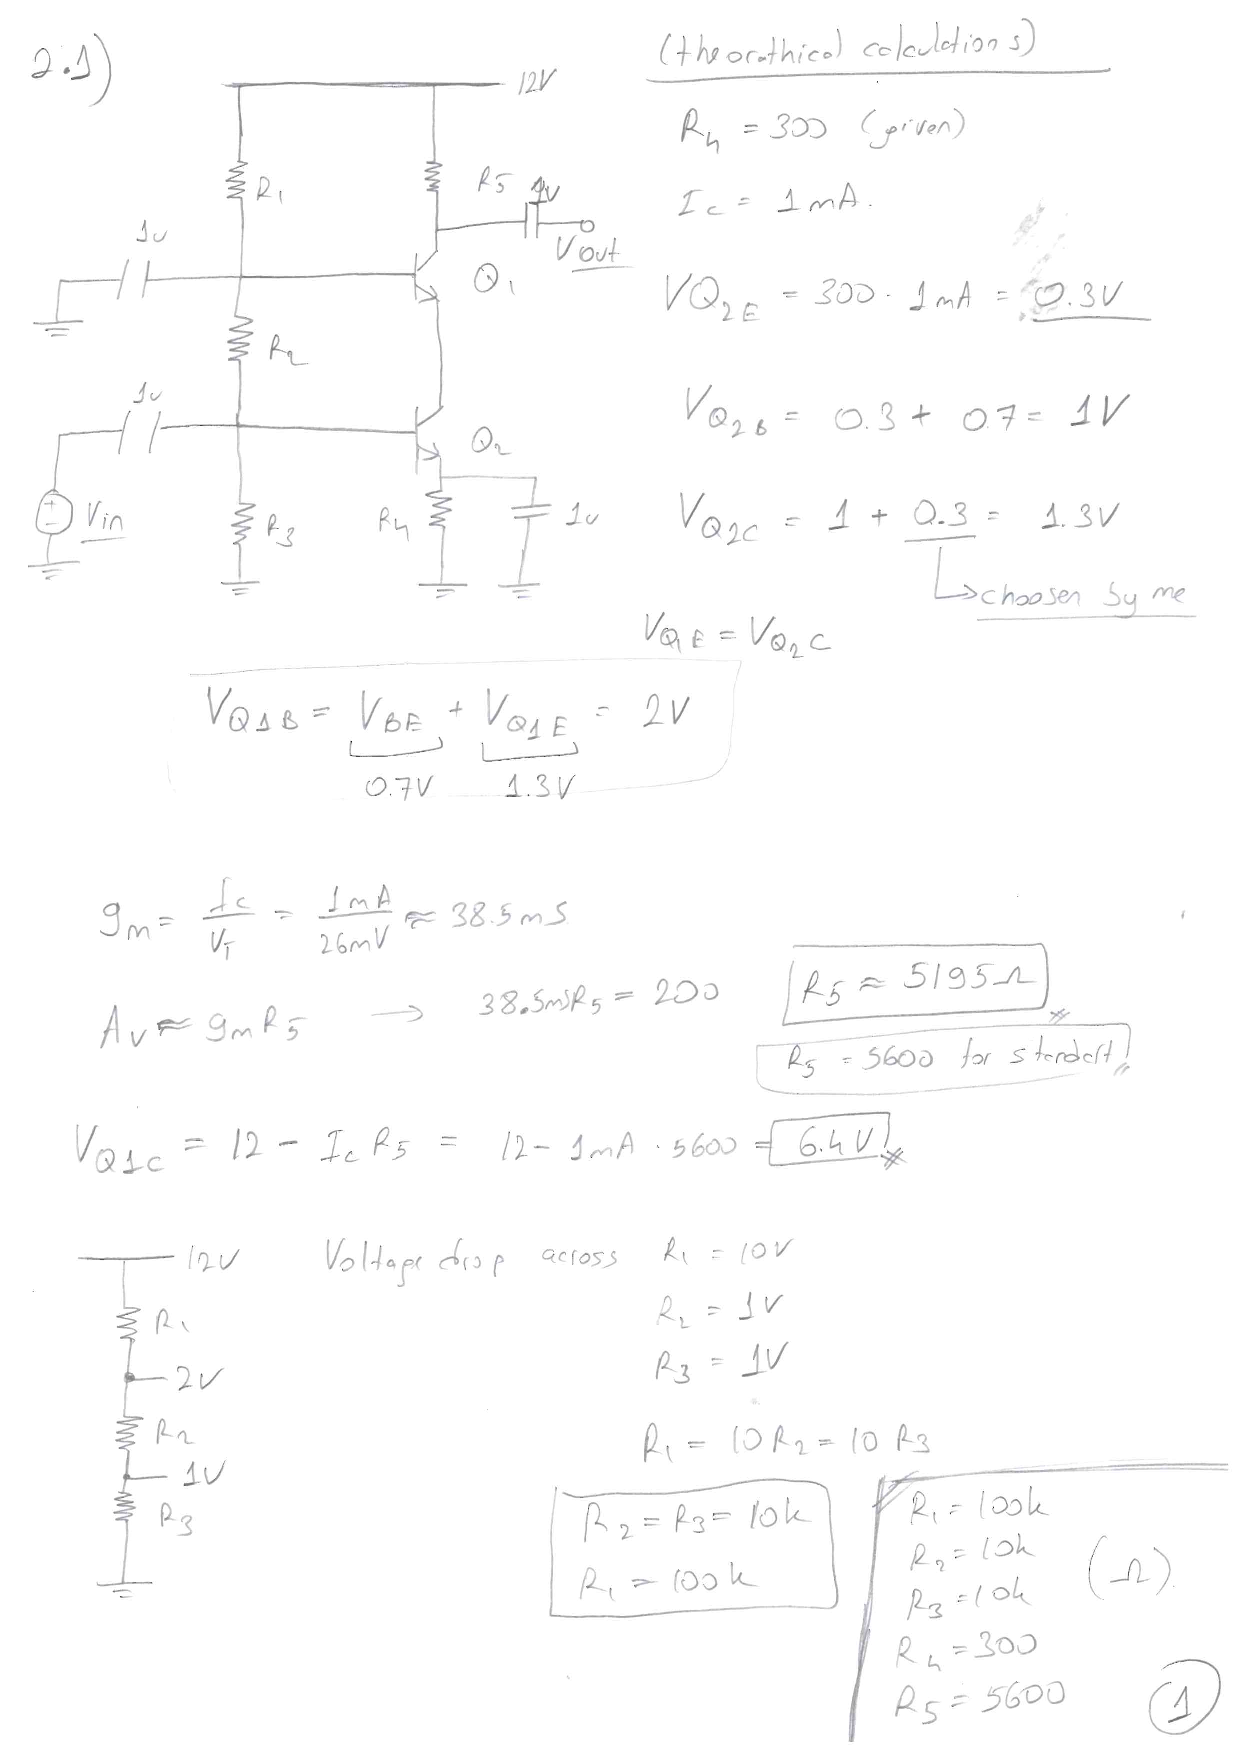
\includepdf[pages=-]{task_2_1.pdf}

\section*{2.2) Simulation and Design Verification}

The cascode amplifier was implemented in LTspice as shown in \textbf{Figure \ref{fig:schematic}}. While the topology was based on the theoretical design from Task 2.1, an iterative tuning process was necessary to account for non-ideal device parameters and base current loading. 

\begin{figure}[H]
    \centering
    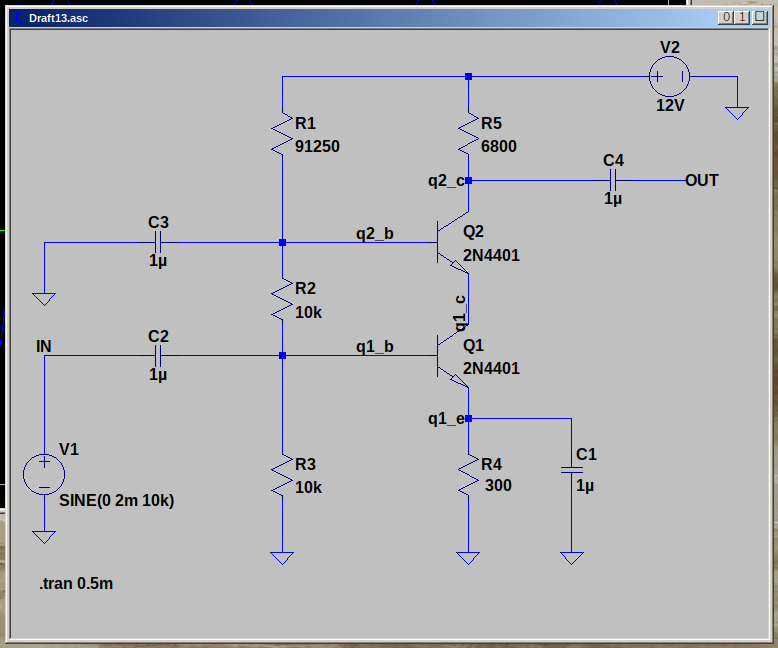
\includegraphics[width=0.75\textwidth]{images/schematic.png} % Replace with your schematic filename
    \caption{Optimized LTspice schematic of the Cascode Amplifier.}
    \label{fig:schematic}
\end{figure}

\subsection*{Gain Measurement}
A transient analysis was conducted using a $2\,mV$ peak sine wave at $10\,kHz$. As shown in \textbf{Figure \ref{fig:gain_plot}}, the output signal at the collector of $Q_2$ exhibited a peak amplitude of $420\,mV$. The voltage gain is calculated as:
\begin{equation}
    A_v = \frac{V_{out(peak)}}{V_{in(peak)}} = \frac{420\,mV}{2\,mV} = 210
\end{equation}
The simulated gain of 210 confirms that the design meets the laboratory requirement of $A_v > 200$.

\begin{figure}[H]
    \centering
    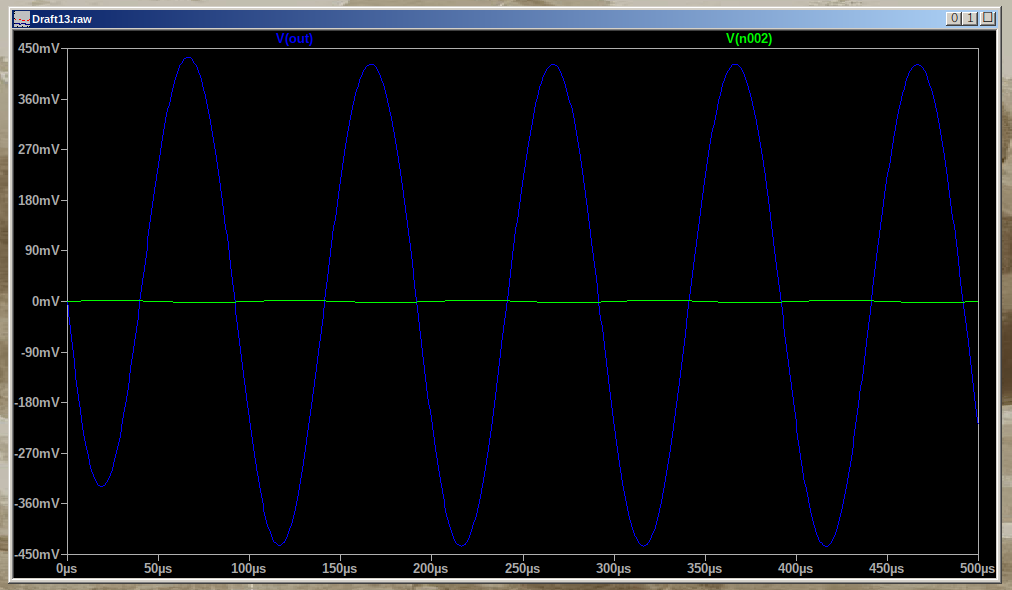
\includegraphics[width=0.8\textwidth]{images/gain_plot.png} % Replace with your gain plot filename
    \caption{Transient analysis showing $V_{in}$ and $V_{out}$ waveforms.}
    \label{fig:gain_plot}
\end{figure}

\subsection*{Input and Output Impedance Measurements}
Using AC small-signal analysis at $10\,kHz$, the input and output impedances were characterized. The results are visualized in \textbf{Figures \ref{fig:zin}} and \textbf{\ref{fig:zout}}.

\begin{itemize}
\item \textbf{Input Impedance ($Z_{in}$):} Measured at the base of $Q_1$, the impedance was found to be approximately $\mathbf{2.44\,k\Omega}$. This value is determined by the parallel combination of the biasing resistors ($R_2 \parallel R_3$) and the transistor's dynamic input resistance ($r_{\pi}$).    \begin{figure}[H]
        \centering
        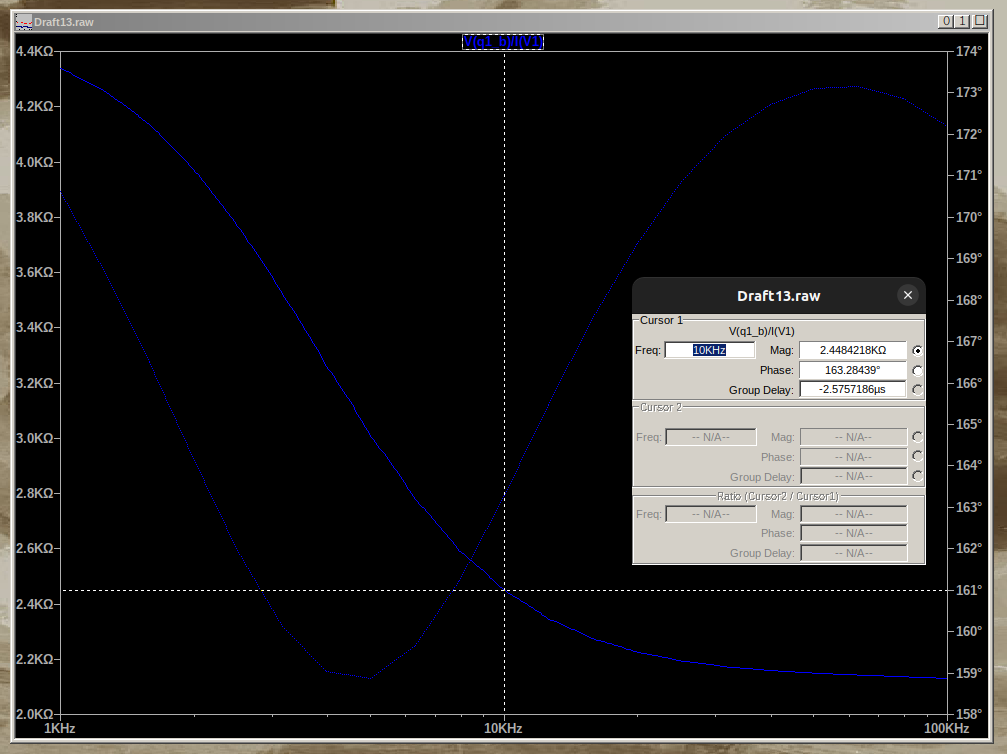
\includegraphics[width=0.8\textwidth]{images/zin.png} % Replace with your Zin filename
        \caption{AC Analysis: Input Impedance.}
        \label{fig:zin}
    \end{figure}
    \item \textbf{Output Impedance ($Z_{out}$):} Measured by probing the output node. The result was approximately $\mathbf{6.8\,k\Omega}$, which is dominated by the load resistor $R_5$.
    \begin{figure}[H]
        \centering
        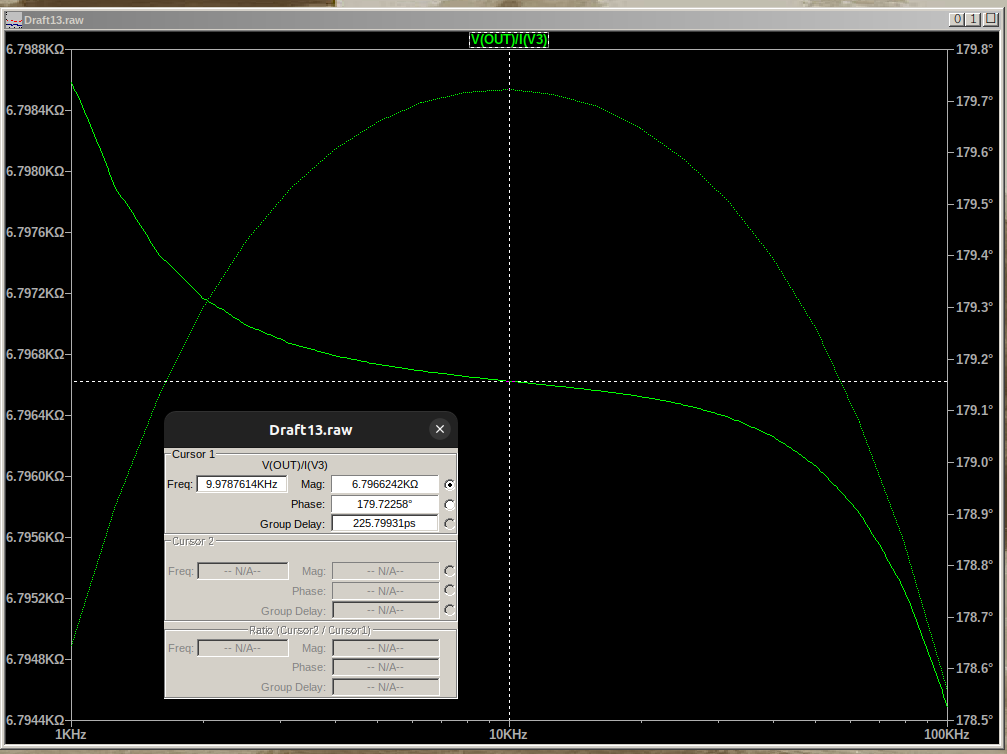
\includegraphics[width=0.8\textwidth]{images/zout.png} % Replace with your Zout filename
        \caption{AC Analysis: Output Impedance.}
        \label{fig:zout}
    \end{figure}
\end{itemize}

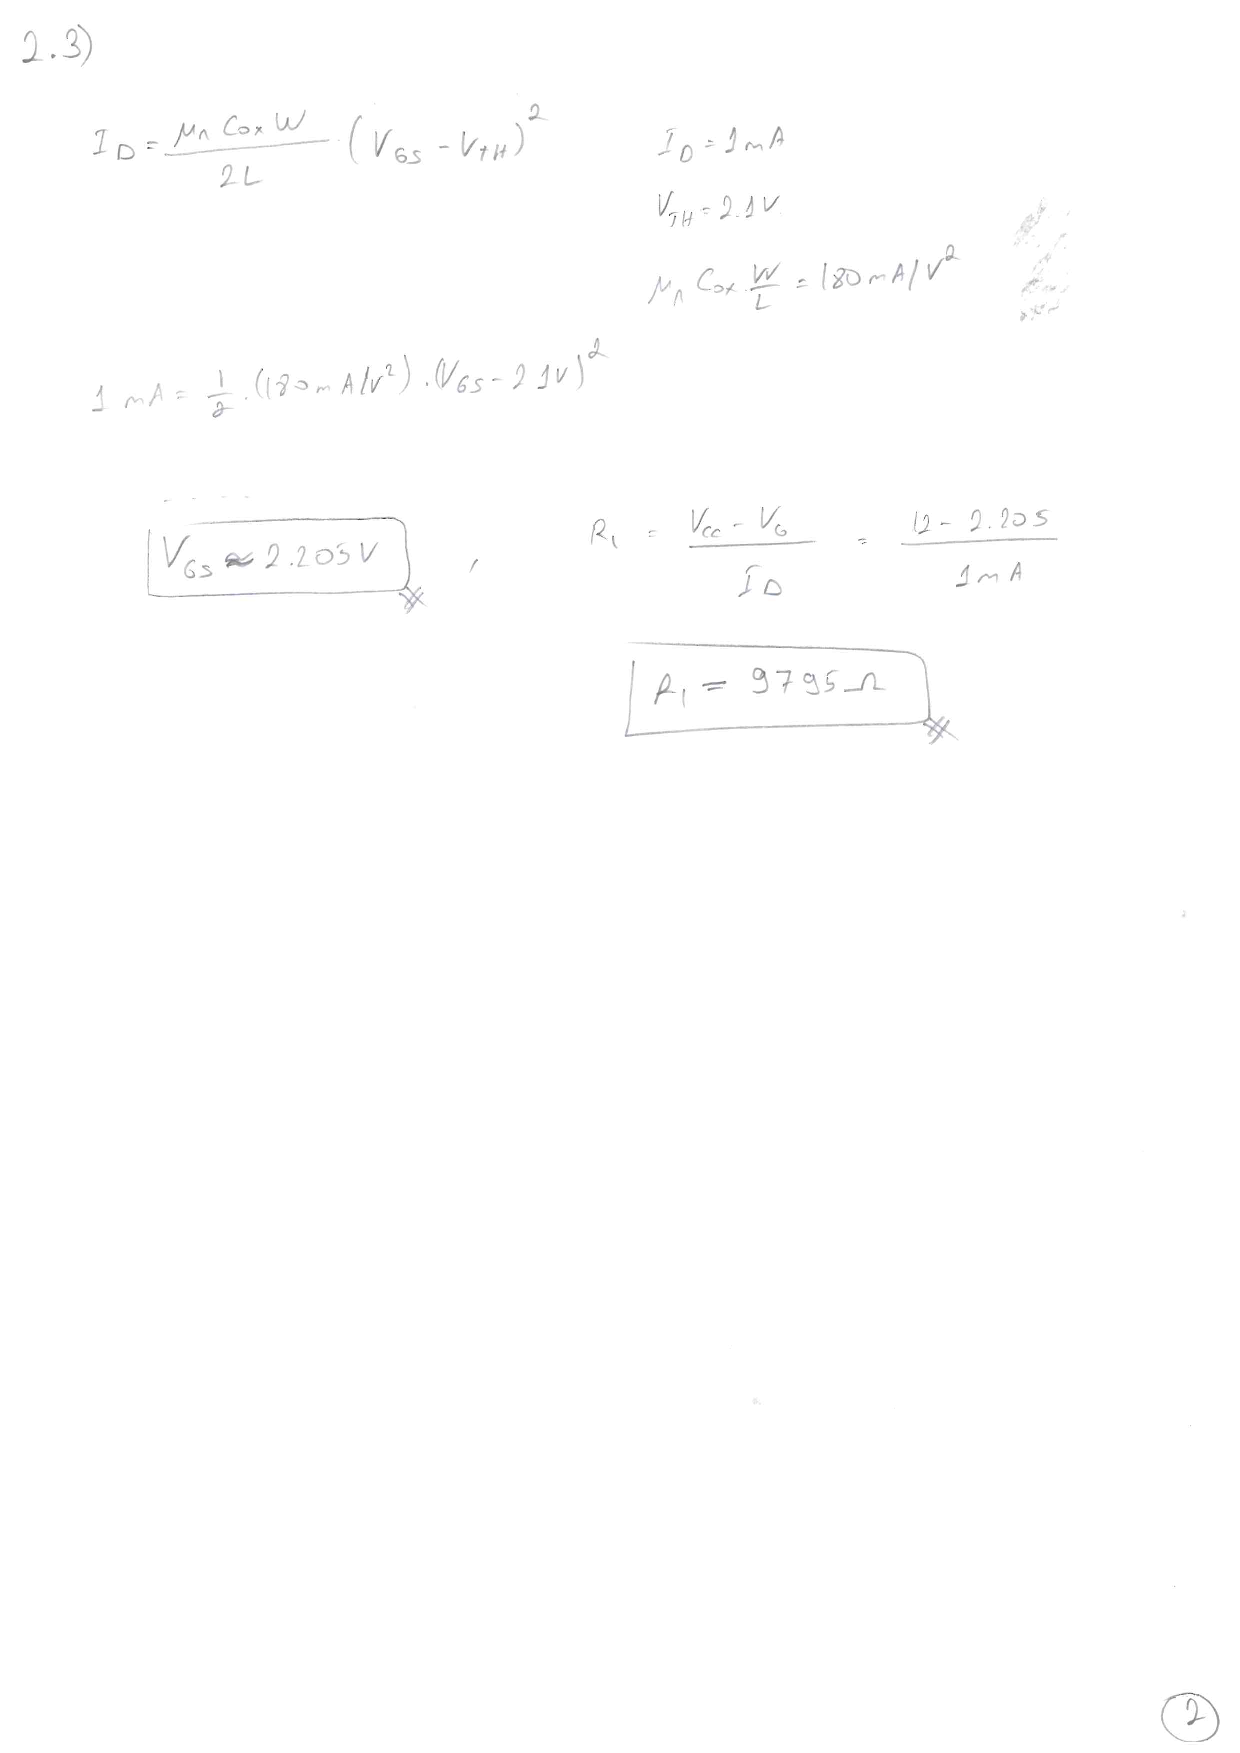
\includepdf{task_2_3.pdf}
\end{document}